\def\usewhat{pdflatex}

% 插入空白页可以设置openright
\documentclass[12pt,openany,oneside]{book}

% 定义本文所使用宏包
%%%%%%%%%% Package %%%%%%%%%%%%

\usepackage{float}
\usepackage{wrapfig}
\usepackage{makecell}
% 支持插图处理
\usepackage{graphicx}
\usepackage[a4paper,text={146.4true mm,239.2 true mm},top= 26.2true mm,left=31.8 true mm,head=6true mm,headsep=6.5true mm,foot=16.5true mm]{geometry}

% 支持版面尺寸设置
% 支持国际标准单位
\usepackage[squaren]{SIunits}               

\usepackage{titlesec}                       % 控制标题的宏包
\usepackage{titletoc}                       % 控制目录的宏包
\usepackage{fancyhdr}                       % fancyhdr宏包 支持页眉和页脚的相关定义
\usepackage[UTF8]{ctex}                     % 支持中文显示
\usepackage{CJKpunct}                       % 精细调整中文的标点符号
\usepackage{color}                          % 支持彩色
\usepackage{amsmath}                        % AMSLaTeX宏包 用来排出更加漂亮的公式
\usepackage{amssymb}                        % 数学符号生成命令
\usepackage[below]{placeins}    %允许上一个section的浮动图形出现在下一个section的开始部分,还提供\FloatBarrier命令,使所有未处理的浮动图形立即被处理
\usepackage{multirow}                       % 使用Multirow宏包,使得表格可以合并多个row格
\usepackage{booktabs}                       % 表格,横的粗线;\specialrule{1pt}{0pt}{0pt}
\usepackage{longtable}                      % 支持跨页的表格。
\usepackage{tabularx}                       % 自动设置表格的列宽
\usepackage{subfigure}                      % 支持子图 %centerlast 设置最后一行是否居中
\usepackage[subfigure]{ccaption}            % 支持子图的中文标题
\usepackage[sort&compress,numbers]{natbib}  % 支持引用缩写的宏包
\usepackage{enumitem}                       % 使用enumitem宏包,改变列表项的格式

\usepackage{calc}                           % 长度可以用+ - * / 进行计算
\usepackage{txfonts}                        % 字体宏包
\usepackage{bm}                             % 处理数学公式中的黑斜体的宏包
\usepackage[amsmath,thmmarks,hyperref]{ntheorem}  % 定理类环境宏包,其中 amsmath 选项用来兼容 AMS LaTeX 的宏包
\usepackage{CJKnumb}                        % 提供将阿拉伯数字转换成中文数字的命令
\usepackage{indentfirst}                    % 首行缩进宏包
\usepackage{CJKutf8}                        % 用在UTF8编码环境下,它可以自动调用CJK,同时针对UTF8编码作了设置
\usepackage{geometry}
\geometry{left=3.0cm,right=2.0cm,top=2.5cm,bottom=2.5cm}
%\usepackage{hypbmsec}                      % 用来控制书签中标题显示内容
\newcommand{\tabincell}[2]{\begin{tabular}{@{}#1@{}}#2\end{tabular}}
\usepackage{xcolor}
%支持代码环境
\usepackage{listings}
\lstset{numbers=left,
language=[ANSI]{C},
numberstyle=\tiny,
extendedchars=false,
showstringspaces=false,
breakatwhitespace=false,
breaklines=true,
captionpos=b,
%keywordstyle=\color{blue!70},
commentstyle=\color{red!50!green!50!blue!50},
%frame=shadowbox,     %阴影边框
%frame=single,          %单线边框
%不加则无边框
rulesepcolor=\color{red!20!green!20!blue!20}
}
%支持算法环境
\usepackage[boxed,ruled,lined]{algorithm2e}
\usepackage{algorithmic}

\usepackage{times}%times字体
\usepackage{lipsum}


\usepackage{array}
\newcommand{\PreserveBackslash}[1]{\let\temp=\\#1\let\\=\temp}
\newcolumntype{C}[1]{>{\PreserveBackslash\centering}p{#1}}
\newcolumntype{R}[1]{>{\PreserveBackslash\raggedleft}p{#1}}
\newcolumntype{L}[1]{>{\PreserveBackslash\raggedright}p{#1}}

% 生成有书签的 pdf 及其生成方式。通常可以在 tjumain.tex 文件的第一行选择 pdflatex 或者是 dvipdfmx 编译手段。如果选择前者,则使用 pdflatex + pdflatex 编译; 如果选择后者,在编译的时候选择 latex + bibtex + latex + latex 编译。出现混淆的时候,系统会报错。
% 如果您的pdf制作中文书签有乱码使用如下命令,就可以解决了
\def\atemp{dvipdfmx}\ifx\atemp\usewhat
\usepackage[dvipdfmx,unicode,               % dvipdfmx 编译, 加入了中文复制,粘贴支持引擎。
            pdfstartview=FitH,
            bookmarksnumbered=true,
            bookmarksopen=true,
            colorlinks=false,
            pdfborder={0 0 1},
            citecolor=blue,
            linkcolor=red,
            anchorcolor=green,
            urlcolor=blue,
            breaklinks=true
            ]{hyperref}
\fi

\def\atemp{pdflatex}\ifx\atemp\usewhat
\usepackage{cmap}                           % pdflatex 编译时,可以生成可复制、粘贴的中文 PDF 文档, 缺点是在Windows上显示时效果不大好,字体发虚
\usepackage[pdftex,unicode,
            %CJKbookmarks=true,
            bookmarksnumbered=true,
            bookmarksopen=true,                       
            hidelinks
%            colorlinks=true,       % original false
%            pdfborder={0 0 1},
%            citecolor=black,       % original blue
%            linkcolor=black,       % original red
%            anchorcolor=black,           % original green
%            urlcolor=blue,
%            breaklinks=false       % original true
            ]{hyperref}
\fi


% 新增for url
\usepackage{url}

%全局设置表格/图片/公式的编号,而不是1.2之类的
\usepackage{remreset}
\makeatletter
\@removefromreset{table}{chapter}
\@removefromreset{figure}{chapter}
\@removefromreset{equation}{chapter}
\makeatother
\renewcommand{\thetable}{\arabic{table}}
\renewcommand{\thefigure}{\arabic{figure}}
\renewcommand{\theequation}{\arabic{equation}}

\newcommand{\chref}[1]{第~\ref{#1}~章}
\newcommand{\secref}[1]{第~\ref{#1}~节}
\newcommand{\figref}[1]{图~\ref{#1}~}
\newcommand{\tabref}[1]{表~\ref{#1}~}
\newcommand{\equaref}[1]{公式~\eqref{#1}~}


% 定义所有的.eps/.pdf图片文件在figure子目录下
\graphicspath{{figure/}}

\begin{document}

% 开始中文字体使用
\begin{CJK*}{UTF8}{song}

% 完成对论文各个部分格式的设置
%%%%%%%%%%%%%%%%% 图片浮动设置 %%%%%%%%%%%%%%%%%
\setcounter{topnumber}{2}
\setcounter{bottomnumber}{2}
\setcounter{totalnumber}{4}
\renewcommand{\topfraction}{0.85}
\renewcommand{\bottomfraction}{0.85}
\renewcommand{\textfraction}{0.15}
\renewcommand{\floatpagefraction}{0.8}
\renewcommand{\textfraction}{0.1}
\setlength{\floatsep}{5pt plus 2pt minus 2pt}
\setlength{\textfloatsep}{5pt plus 2pt minus 2pt}
\setlength{\intextsep}{5pt plus 2pt minus 2pt}

%%%%%%%%%%%%%%%%% Fonts Definition and Basics %%%%%%%%%%%%%%%%%
\newcommand{\song}{\CJKfamily{song}}    % 宋体
\newcommand{\fs}{\CJKfamily{fs}}        % 仿宋体
\newcommand{\kai}{\CJKfamily{kai}}      % 楷体
\newcommand{\hei}{\CJKfamily{hei}}      % 黑体
\newcommand{\li}{\CJKfamily{li}}        % 隶书
\newcommand{\chuhao}{\fontsize{28pt}{28pt}\selectfont}       % 初号, 单倍行距
\newcommand{\yihao}{\fontsize{26pt}{26pt}\selectfont}       % 一号, 单倍行距
\newcommand{\xiaoyi}{\fontsize{24pt}{24pt}\selectfont}      % 小一, 单倍行距
\newcommand{\erhao}{\fontsize{22pt}{1.25\baselineskip}\selectfont}       % 二号, 1.25倍行距
\newcommand{\xiaoer}{\fontsize{18pt}{18pt}\selectfont}      % 小二, 单倍行距
\newcommand{\sanhao}{\fontsize{16pt}{16pt}\selectfont}      % 三号, 单倍行距
\newcommand{\xiaosan}{\fontsize{15pt}{15pt}\selectfont}     % 小三, 单倍行距
\newcommand{\sihao}{\fontsize{14pt}{14pt}\selectfont}       % 四号, 单倍行距
\newcommand{\xiaosi}{\fontsize{12pt}{12pt}\selectfont}      % 小四, 单倍行距
\newcommand{\wuhao}{\fontsize{10.5pt}{10.5pt}\selectfont}   % 五号, 单倍行距
\newcommand{\xiaowu}{\fontsize{9pt}{9pt}\selectfont}        % 小五, 单倍行距

% 重新定义了波浪符~的意义
\CJKtilde

% 定义章的pre-post名称
\newcommand\prechaptername{第}
\newcommand\postchaptername{章}

% 调整中文字符的表示,行内占一个字符宽度,行尾占半个字符宽度
% 行末半角?
\punctstyle{hangmobanjiao}             

% 调整罗列环境的布局
\setitemize{leftmargin=3em,itemsep=0em,partopsep=0em,parsep=0em,topsep=-0em}
\setenumerate{leftmargin=3em,itemsep=0em,partopsep=0em,parsep=0em,topsep=0em,label={(\arabic*)}}

% 避免宏包 hyperref 和 arydshln 不兼容带来的目录链接失效的问题。
\def\temp{\relax}
\let\temp\addcontentsline
\gdef\addcontentsline{\phantomsection\temp}

% 自定义项目列表标签及格式 \begin{publist} 列表项 \end{publist}
\newcounter{pubctr} %自定义新计数器
\newenvironment{publist}{%%%%%定义新环境
\begin{list}{[\arabic{pubctr}]} %%标签格式
    {
     \usecounter{pubctr}
     \setlength{\leftmargin}{2.5em}   % 左边界 \leftmargin =\itemindent + \labelwidth + \labelsep
     \setlength{\itemindent}{0em}     % 标号缩进量
     \setlength{\labelsep}{1em}       % 标号和列表项之间的距离,默认0.5em
     \setlength{\rightmargin}{0em}    % 右边界
     \setlength{\topsep}{0ex}         % 列表到上下文的垂直距离
     \setlength{\parsep}{0ex}         % 段落间距
     \setlength{\itemsep}{0ex}        % 标签间距
     \setlength{\listparindent}{0pt}  % 段落缩进量
    }}
{\end{list}}

\makeatletter
	\renewcommand\normalsize{
		\@setfontsize\normalsize{12pt}{12pt} % 小四对应 12 pt
		\setlength\abovedisplayskip{4pt}
		\setlength\abovedisplayshortskip{4pt}
		\setlength\belowdisplayskip{\abovedisplayskip}
		\setlength\belowdisplayshortskip{\abovedisplayshortskip}
		\let\@listi\@listI}
	
	% 不同的行距设置
	% TJU原始值1.63
	% 设为1.8则一页31行,1.95则一页29行(目前采用值)(约1.5倍行距)
	\def\defaultfont{\renewcommand{\baselinestretch}{1.95}\normalsize\selectfont} % 设置行距,正文一页29行
	
	% 控制字间距,使每行 34 个汉字
	\renewcommand{\CJKglue}{\hskip -0.1 pt plus 0.08\baselineskip} 
\makeatother

%%%%%%%%%%%%% Contents 目录 %%%%%%%%%%%%%%%%%

\renewcommand{\contentsname}{目录}

% 控制目录深度,改为1
\setcounter{tocdepth}{1}

\titlecontents{chapter}[2em]{\vspace{.0\baselineskip}\xiaosi\song}	% 可以重调skip
	{\prechaptername\CJKnumber{\thecontentslabel}\postchaptername\quad}{}
	{\!\titlerule*[5pt]{$\cdot$}\!\!\!\!\xiaosi\contentspage}	% 调整点的距离
\titlecontents{section}[3em]{\vspace{-0.1\baselineskip}\xiaosi\song}
	{\thecontentslabel\quad}{}
	{\!\titlerule*[5pt]{$\cdot$}\!\!\!\!\xiaosi\contentspage}
\titlecontents{subsection}[4em]{\vspace{-0.2\baselineskip}\xiaosi\song}
	{\thecontentslabel\quad}{}
	{\!\titlerule*[5pt]{$\cdot$}\!\!\!\!\xiaosi\contentspage}
             
%%%%%%%%%% Chapter and Section 章节 %%%%%%%%%%%%%

\setcounter{secnumdepth}{4}
\setlength{\parindent}{2em}

% 如果使用第“一”章
\renewcommand{\chaptername}{\prechaptername\CJKnumber{\thechapter}\postchaptername}
% 使用第“1”章
%\renewcommand{\chaptername}{\thechapter}

% 此处修改的chapter title会被主文件定义覆盖
% chapter标题格式:小二,黑体,居中
\titleformat{\chapter}{\centering\xiaoer\hei}{\chaptername}{2em}{}
\titlespacing{\chapter}{0pt}{0.1\baselineskip}{0.8\baselineskip}

% section标题格式:四号,黑体,左对齐
\titleformat{\section}{\sihao\hei}{\thesection}{1em}{}
\titlespacing{\section}{0pt}{0.15\baselineskip}{0.25\baselineskip}

% subsection标题格式:小四,黑体,左对齐
\titleformat{\subsection}{\xiaosi\hei}{\thesubsection}{1em}{}
\titlespacing{\subsection}{0pt}{0.1\baselineskip}{0.3\baselineskip}

% subsubsection标题格式:小四,宋体加粗,左对齐
\titleformat{\subsubsection}{\xiaosi\song\bfseries}{\thesubsubsection}{1em}{}
\titlespacing{\subsubsection}{0pt}{0.05\baselineskip}{0.1\baselineskip}

%%%%%%%%%% Table, Figure and Equation 图/表/公式 %%%%%%%%%%%%%%%%%

\renewcommand{\tablename}{表}
\renewcommand{\figurename}{图}

% 使图编号为 7-1 的格式
%\renewcommand{\thefigure}{\arabic{chapter}-\arabic{figure}}
%按顺序编号
%\renewcommand{\thefigure}{\arabic{figure}}
% 使子图编号为 a) 的格式
%\renewcommand{\thesubfigure}{\alph{subfigure})}
% 使子图编号为 (a) 的格式
\renewcommand{\thesubfigure}{(\alph{subfigure})}

% 使子表编号为 (a) 的格式
\renewcommand{\thesubtable}{(\alph{subtable})}
% 使表编号为 7-1 的格式
%\renewcommand{\thetable}{\arabic{chapter}-\arabic{table}}
%按顺序编号
\renewcommand{\thetable}{\arabic{table}}
% 使公式编号为 7-1 的格式
%\renewcommand{\theequation}{\arabic{chapter}-\arabic{equation}}

\makeatletter
	% 使子图引用也是7-1a)或7-1(a)的形式
	\renewcommand{\p@subfigure}{\thefigure}
\makeatother

% 定制浮动图形和表格标题样式
\makeatletter
	\long\def\@makecaption#1#2{
	   \vskip\abovecaptionskip
	   \sbox\@tempboxa{\centering\wuhao\song\bfseries{#1\quad #2}}
	   \ifdim \wd\@tempboxa >\hsize
	     \centering\wuhao\song{#1\quad #2} \par	% narrower
	   \else
	     \global \@minipagefalse
	     \hb@xt@\hsize{\hfil\box\@tempboxa\hfil}
	   \fi
	   \vskip\belowcaptionskip}
\makeatother

% 用来控制longtable表头分隔符
\captiondelim{~~~~} 

%%%%%%%%%% Theorem Environment 定理 %%%%%%%%%%%%%%%%%
\theoremstyle{plain}
\theorembodyfont{\song\rmfamily}
\theoremheaderfont{\hei\rmfamily}
\newtheorem{theorem}{定理~}[chapter]
\newtheorem{lemma}{引理~}[chapter]
\newtheorem{axiom}{公理~}[chapter]
\newtheorem{proposition}{命题~}[chapter]
\newtheorem{prop}{性质~}[chapter]
\newtheorem{corollary}{推论~}[chapter]
\newtheorem{conclusion}{结论~}[chapter]
\newtheorem{definition}{定义~}[chapter]
\newtheorem{conjecture}{猜想~}[chapter]
\newtheorem{example}{例~}[chapter]
\newtheorem{remark}{注~}[chapter]
%\newtheorem{algorithm}{算法~}[chapter]
\newenvironment{proof}{\noindent{\hei 证明:}}{\hfill $ \square $ \vskip 4mm}
\theoremsymbol{$\square$}

%%%%%%%%%% Page: number, header and footer 页面设置 %%%%%%%%%%%%%%%%%

%\frontmatter 或 \pagenumbering{roman}
%\mainmatter 或 \pagenumbering{arabic}

\makeatletter
	\renewcommand\frontmatter{\clearpage
		\@mainmatterfalse}
\makeatother

%%%%%%%%%%%% References 参考文献 %%%%%%%%%%%%%%%%%

\renewcommand{\bibname}{参考文献}
% 重定义参考文献样式,来自thu
\makeatletter
\renewenvironment{thebibliography}[1]{
    %\titleformat{\chapter}{\raggedright\sihao\hei}{\chaptername}{2em}{}
    %\titleformat{\chapter}{\centering\sihao\hei}{\chaptername}{2em}{}
    %\titleformat{\chapter}{\centering\xiaoer\hei}{\chaptername}{2em}{}
   \chapter*{\bibname}
   \xiaosi
   \list{\@biblabel{\@arabic\c@enumiv}}
        {\renewcommand{\makelabel}[1]{##1\hfill}
         \settowidth\labelwidth{0 cm}
         \setlength{\labelsep}{0pt}
         \setlength{\itemindent}{0pt}
         \setlength{\leftmargin}{\labelwidth+\labelsep}
         \addtolength{\itemsep}{-0.7em}
%         \addtolength{\itemsep}{-1.0em}
         \linespread{1.5}\selectfont	% 调整每个参考文献项内的间距 !!!
         \usecounter{enumiv}
         \let\p@enumiv\@empty
         \renewcommand\theenumiv{\@arabic\c@enumiv}}
    \sloppy\frenchspacing
    \clubpenalty4000
    \@clubpenalty \clubpenalty
    \widowpenalty4000
    \interlinepenalty4000
    \sfcode`\.\@m}
   {\def\@noitemerr
     {\@latex@warning{Empty `thebibliography' environment}}
    \endlist\frenchspacing}
\makeatother

% 缩小参考文献间的垂直间距
\addtolength{\bibsep}{-0.5em}

% 每个条目自第二行起缩进的距离
\setlength{\bibhang}{2em}

% 参考文献引用作为上标出现
\makeatletter
	\def\@cite#1#2{\textsuperscript{[{#1\if@tempswa , #2\fi}]}}
\makeatother

% 引用格式
\bibpunct{[}{]}{,}{s}{}{,}

%%%%%%%%%%%% Cover 封面、摘要、版权、致谢格式定义 %%%%%%%%%%%%%%%%%
 
\makeatletter % 一直到结尾

\def\ctitle#1{\def\@ctitle{#1}}\def\@ctitle{}
\def\etitle#1{\def\@etitle{#1}}\def\@etitle{}
\def\subtitle#1{\def\@subtitle{#1}}\def\@subtitle{}
\def\esubject#1{\def\@esubject{#1}}\def\@esubject{}
\def\cauthor#1{\def\@cauthor{#1}}\def\@cauthor{}
\def\eauthor#1{\def\@eauthor{#1}}\def\@eauthor{}
\def\csupervisor#1{\def\@csupervisor{#1}}\def\@csupervisor{}
\def\esupervisor#1{\def\@esupervisor{#1}}\def\@esupervisor{}
\def\cdate#1{\def\@cdate{#1}}\def\@cdate{}
\long\def\cabstract#1{\long\def\@cabstract{#1}}\long\def\@cabstract{}
\long\def\eabstract#1{\long\def\@eabstract{#1}}\long\def\@eabstract{}
\def\ckeywords#1{\def\@ckeywords{#1}}\def\@ckeywords{}
\def\ekeywords#1{\def\@ekeywords{#1}}\def\@ekeywords{}
\def\cheading#1{\def\@cheading{#1}}\def\@cheading{北京航空航天大学第三十二届“冯如杯”竞赛主赛道参赛作品}

\pagestyle{fancy}
  \fancyhf{}
  \fancyhead[C]{\song\wuhao \@cheading}  % 页眉
%  \lhead{\song\wuhao \@cheading}  % 左页眉
%  \rhead{\prechaptername\CJKnumber{\thechapter}\postchaptername}    % 右页眉
%  \rhead{\prechaptername~\thechapter~\postchaptername}    % 右页眉
  \fancyfoot[C]{\song\xiaowu ~\thepage~}
\newlength{\@title@width}

% 定义封面
\def\makecover{
   \phantomsection
    \pdfbookmark[-1]{\@ctitle}{ctitle}

%%%%%%%%%%%%%%%%%%% Abstract and Keywords 摘要和关键词 %%%%%%%%%%%%%%%%%%%%%%%

%中文摘要格式
\clearpage
\markboth{摘要}{摘要}
\pdfbookmark[0]{摘要}{cabstract}

% 摘要不加到目录中
%\addcontentsline{toc}{chapter}{摘要}

% 开始罗马数字编号
\setcounter{page}{1}
\pagenumbering{roman}
\thispagestyle{plain}


% 中文摘要:小二,黑体加粗,居中
\begin{center}
% \xiaosan\hei\bfseries 摘要
\xiaosan\hei 摘要
\end{center}

%\vspace{\baselineskip} % 新增摘要后空行

% 插入中文摘要
\song\defaultfont
\@cabstract
% \vspace{\baselineskip}

%\hangafter=1\hangindent=52.3pt\noindent
\hangafter=1\hangindent=52.3pt
{\song\xiaosi 关键词:} \@ckeywords
%\thispagestyle{empty}

% 英文摘要格式
\clearpage
 \markboth{Abstract}{Abstract}
 \pdfbookmark[0]{Abstract}{eabstract}

 % 摘要不加到目录中
 %\addcontentsline{toc}{chapter}{ABSTRACT}

 \thispagestyle{plain}

% ABSTRACT三号居中
 \begin{center}
 % \sanhao{\bf{Abstract}}
 \sanhao{Abstract}
 \end{center}
% \vspace{\baselineskip}

% 插入英文摘要
\@eabstract
% \vspace{\baselineskip}

% \hangafter=1\hangindent=60pt\noindent
\hangafter=1\hangindent=60pt
{\textbf{Keywords:}} \@ekeywords
\thispagestyle{plain}

}
\makeatother
     

% ——————————————————————————————————————————————
% 以下是论文导言部分,包括论文的封面,中英文摘要和中文目录

\frontmatter
\fancypagestyle{plain}{
\fancyhf{}
\renewcommand{\headrulewidth}{0 pt}

\fancyfoot[C]{\wuhao\thepage}
}

%%%%%%%%%%   封面   %%%%%%%%%%

\begin{titlepage}

\newcommand{\HRule}{\rule{\linewidth}{0.5mm}} % Defines a new command for the horizontal lines, change thickness here

\center % Center everything on the page
 
%----------------------------------------------------------------------------------------
%	HEADING SECTIONS
 %----------------------------------------------------------------------------------------

\textsc{\LARGE  北京航空航天大学}\\[1.5cm] % Name of your university/college

\includegraphics[scale=0.9]{figure/buaa_logo.png}\\[1cm] % Include a department/university logo - this will require the graphicx package
\textsc{\Large 冯如杯}\\[0.5cm] % Major heading such as course name
%\textsc{\large Course code}\\[0.5cm] % Minor heading such as course title

%----------------------------------------------------------------------------------------
%	TITLE SECTION
%----------------------------------------------------------------------------------------

\HRule \\[1cm]
{ \huge  \bfseries PhoeniX}\\[0.4cm] % Title of your document
\HRule \\[1cm]
 
%----------------------------------------------------------------------------------------
%	AUTHOR SECTION
%----------------------------------------------------------------------------------------

\begin{minipage}{0.4\textwidth}
\begin{center} \large

% \begin{flushleft}
%     \quad \quad \quad \emph{作者:}\\
% \end{flushleft}

% First name \textsc{Last name}\\ % Your name
\begin{align*}
    \emph{}& \text{}\\
    \emph{}& \text{}\\
\end{align*}
\end{center}

\end{minipage}\\[2cm]

% If you don't want a supervisor, uncomment the two lines below and remove the section above
%\Large \emph{Author:}\\
%John \textsc{Smith}\\[3cm] % Your name

%----------------------------------------------------------------------------------------
%	DATE SECTION
%----------------------------------------------------------------------------------------

{\large \today}\\[2cm] % Date, change the \today to a set date if you want to be precise

\vfill % Fill the rest of the page with whitespace

\end{titlepage}



%%%%%%%%%%   摘要   %%%%%%%%%%

\cabstract{

    “刷题”对于每一名计算机专业的学生而言无疑是重要的,不仅它可以扎实学生的编程基础,而且面试企业工作首先就要用题来考查面试者。但是目前市面上的在线评测系统大多存在着一定的缺陷,由于采用集中评测制,不能良好的应对不定期的大流量评测事件,例如举办特定的比赛。此外,该类系统的功能大多单一,用户在实现刷题后很难与其他用户进行交流心得,或是发布自己的教程。
    
    为此,我们提出了基于Electron-Vue+Gin框架的轻量级、分布式、All-in-one的分布式综合性学习平台。本系统内置了相当多的题目供用户作答。由于采用了分布式部署的策略,评测阶段将会在客户端运行,用户仅需将评测结果上传至云端,相较于传统评测系统大大增加了系统的并发量。可以良好的应对各种大型比赛活动的评测。此外,为了增加用户之间的知识共享,我们还设置了讨论区与教程区,用户可以在里面自由发表观点与对题目的建议互相讨论题目,并在教程区发表一系列教程来发表自己对于某一块知识的理解供其他用户交流学习。
}

\ckeywords{分布式,在线评测,开源软件}

\eabstract{
    "Coding" for every computer major students is undoubtedly important, not only it can solid programming foundation of students, but also the interview of enterprise work must first use the question to examine the interviewer.  However, most of the online evaluation systems on the market have some defects. Because of the centralized evaluation system, they can not cope with the irregular large-scale evaluation events, such as holding specific competitions.  In addition, most of the functions of this system are single, so it is difficult for users to communicate with other users or publish their own tutorials.
    
    Therefore, we propose a lightweight, distributed, all-in-one distributed comprehensive learning platform based on the Electron-Vue+Gin framework.  This system has built in quite a number of questions for users to answer.  Due to the distributed deployment strategy, the evaluation phase will run on the client side, and users only need to upload the evaluation results to the cloud, which greatly increases the concurrency of the system compared with the traditional evaluation system.  Can deal with the evaluation of various large-scale competition activities.  In addition, in order to increase knowledge sharing among users, we also set up discussion area and tutorial area, where users can freely express their views and suggestions on topics and discuss topics with each other, and publish a series of tutorials in the tutorial area to express their understanding of a certain piece of knowledge for other users to exchange and learn.
}

\ekeywords{Distributed, Online judge, Open source software}

\makecover

\clearpage



%%%%%%%%%%   目录   %%%%%%%%%%
\defaultfont
%\clearpage{\pagestyle{empty}\cleardoublepage}
\clearpage
%\pagestyle{empty}
%\setcounter{page}{1}                                 % 单独从 1 开始编页码
%\pagenumbering{arabic}
\titleformat{\chapter}{\centering\sanhao\song}{\chaptername}{2em}{} % 设置目录两字的格式

\tableofcontents                                     % 中文目录


\thispagestyle{plain}

% ——————————————————————————————————————————————
% 以下是论文正文,内容在body子文件夹下

\mainmatter\defaultfont\sloppy\raggedbottom
\makeatletter
	\fancypagestyle{plain}{                              % 设置开章页眉页脚风格
		\fancyhf{}
		\fancyhead[C]{\song\wuhao \@cheading}            % 首页页眉格式
		\fancyfoot[C]{\song\wuhao ~\thepage~}           % 首页页脚格式
		\renewcommand{\headrulewidth}{0.5pt}
		\renewcommand{\footrulewidth}{0pt}}
\makeatother


% 单独从 1 开始编页码
\setcounter{page}{1}
% chapter标题格式:三号,黑体,左对齐
\titleformat{\chapter}{\centering\sanhao\hei}{\chaptername}{2em}{}

%%%%%%%%%%   正文   %%%%%%%%%%

\chapter{引言}

\section{项目背景}
在线评测(Online Judge,下文简称为OJ)系统是用于编程练习的平台,用户可以在平台上搜索相关的编程题目,并在线提交自己的答案(即C、Python、JavaScript等语言的源代码)。OJ系统会对这些源代码进行编译和执行,并通过预先设计的测试数据来评测程序源代码的正确性,最后将评测结果呈现给用户。

OJ系统最初使用于ACM-ICPC国际大学生程序设计竞赛和OI信息学奥林匹克竞赛中的自动判题和排名。现广泛应用于世界各地高校学生程序设计的训练、参赛队员的训练和选拔、各种程序设计竞赛以及数据结构和算法的学习和作业的自动提交判断中。北航软件学院的AC编程平台就是一个传统的OJ系统,程序设计基础、大学计算机基础等北航校内的课程都依托于AC编程平台开展。

但是,传统的OJ系统仍然存在着许多局限性:它通常以黑盒测试的形式判定程序的正确性,简单地给用户呈现通过的测试用例的数量,不检查用户的代码质量。它通常也仅能对单文件的源代码进行评测,不能对多文件的项目进行评测。目前市面上虽然有极少数的OJ系统(如北航编译原理课程使用的rurikawa系统)支持多文件的评测,但这些OJ系统不能支撑有一定并发量的评测。当遇到多个用户同时评测的情况时,这些OJ系统的评测队列会非常拥挤,用户需要等待极长的时间才能获得评测的结果。另外,传统的OJ平台太过纯粹了,用户只能在OJ平台上验证已知的知识,而新知识的获取则需另寻他途,用户经常需要在互联网的海洋中搜索许久才能领会到某个编程练习的背景知识。

\begin{figure}[H]
    \centering
    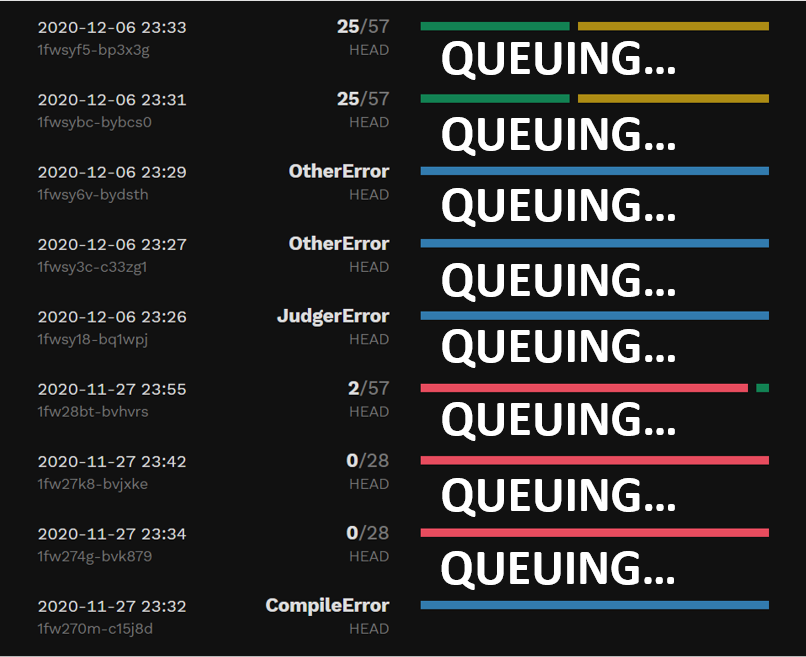
\includegraphics[width=0.7\textwidth]{figure/queuing.png}
    \caption{\textbf{传统OJ系统拥挤的评测队列}}
    \label{fig:queuing}
\end{figure}

\section{项目概述}

PhoeniX是一体化的编程学习平台,旨在为编程学习的相关课程以及编程学习者提供服务。在PhoeniX平台上,用户可以搜索并查阅特定方向的教程和题目,选择题目进行练习并检测自己编写的程序的正确性。用户可以自发地成立组织,在组织内进行教程与题目的发布、共享相关资源、举办范围性的比赛、进行相关讨论……PhoeniX还能基于用户的评测结果以及大数据的统计分析结果,给用户推荐合适的教程与题目,帮助用户提高技术水平与编程能力。

相比于传统的OJ平台,PhoeniX支持对多文件的项目进行评测,打破了传统OJ平台单文件评测的限制,解决了人工手动运行、评测项目级代码的痛点问题。PhoeniX还创新性地将评测过程转移到了用户端,有效降低了用户的评测等待时间,同时大幅减少了远程服务器的资源消耗,可以良好地应对各种大型比赛活动的评测需求,非常适合成本有限的课堂教学环境。另外,PhoeniX还解决了传统OJ平台的内容过于纯粹的问题,PhoeniX在题目评测的基础上加入了资源共享、轻社交、交互式教程等元素,提供了完整的的编程学习服务。

\section{项目创新点与先进性}

\begin{enumerate}
    \item 将传统OJ平台的评测过程转移到用户端进行,采用分布式评测的思想,极大地减少了用户评测的等待时间,提高了用户体验。
    \item 基于Electron框架开发,支持跨平台使用。PhoeniX项目的客户端在Windows、Linux和Mac OS等操作系统上均可使用,全平台数据互通。
    \item 支持对含有多文件、具有复杂目录结构的项目进行评测,在理论上能够支持几乎所有类型的项目评测,打破了传统OJ的单文件评测限制。
    \item 支持对Java、Python、JavaScript、C++、Golang等多语言的评测。可以自定义配置编译和运行的命令,以支持任何编程语言。
    \item 用户可以自行发布题目和教程。PhoeniX允许用户使用Markdown语法与Latex语法进行题目与教程的编写,支持嵌入可交互式的代码执行环境。
    \item 提供组织管理功能,用户可以自行创建组织。在组织内,用户可以开展比赛、在组织论坛内进行讨论、共享组织的题目与教程。
    \item 提供教程和题目的智能推荐,PhoeniX可以给用户推荐最适合用户的题目和教程,提高用户的学习体验。
\end{enumerate}

\section{项目难点与解决方案}

\begin{enumerate}
    \item 如何在用户机上向目标程序调用编译、执行的相关命令?\\
          利用Node.js的相关多进程API创建子进程,父子进程之间采用管道通信。
    \item 如何将输入数据传给目标程序,并获取到目标程序的输出?\\
          将子进程的输入输出进行重定向,将用户程序的输出转存到文件中。
    \item 如何在支持Markdown语法的同时,渲染代码的可执行环境?\\
          使用markdown-it渲染器作为Markdown文本的基础渲染器,并编写相关插件嵌入Visual Studio Code类似风格的代码执行环境。
    \item 如何判断用户程序已执行超时?\\
          利用Node.js的相关多进程API,设定子进程的运行时间限制,当到达限定时间时子进程返回特定的退出码。
    \item 如何实现PhoeniX的跨平台构建?\\
          在CI/CD工作流中将构建分为Windows构建、Linux构建、Mac OS构建三个任务,利用Github Actions进行自动构建。
\end{enumerate}
\newpage
\chapter{系统架构}

\section{桌面端架构}

\begin{figure}[H]
  \centering
  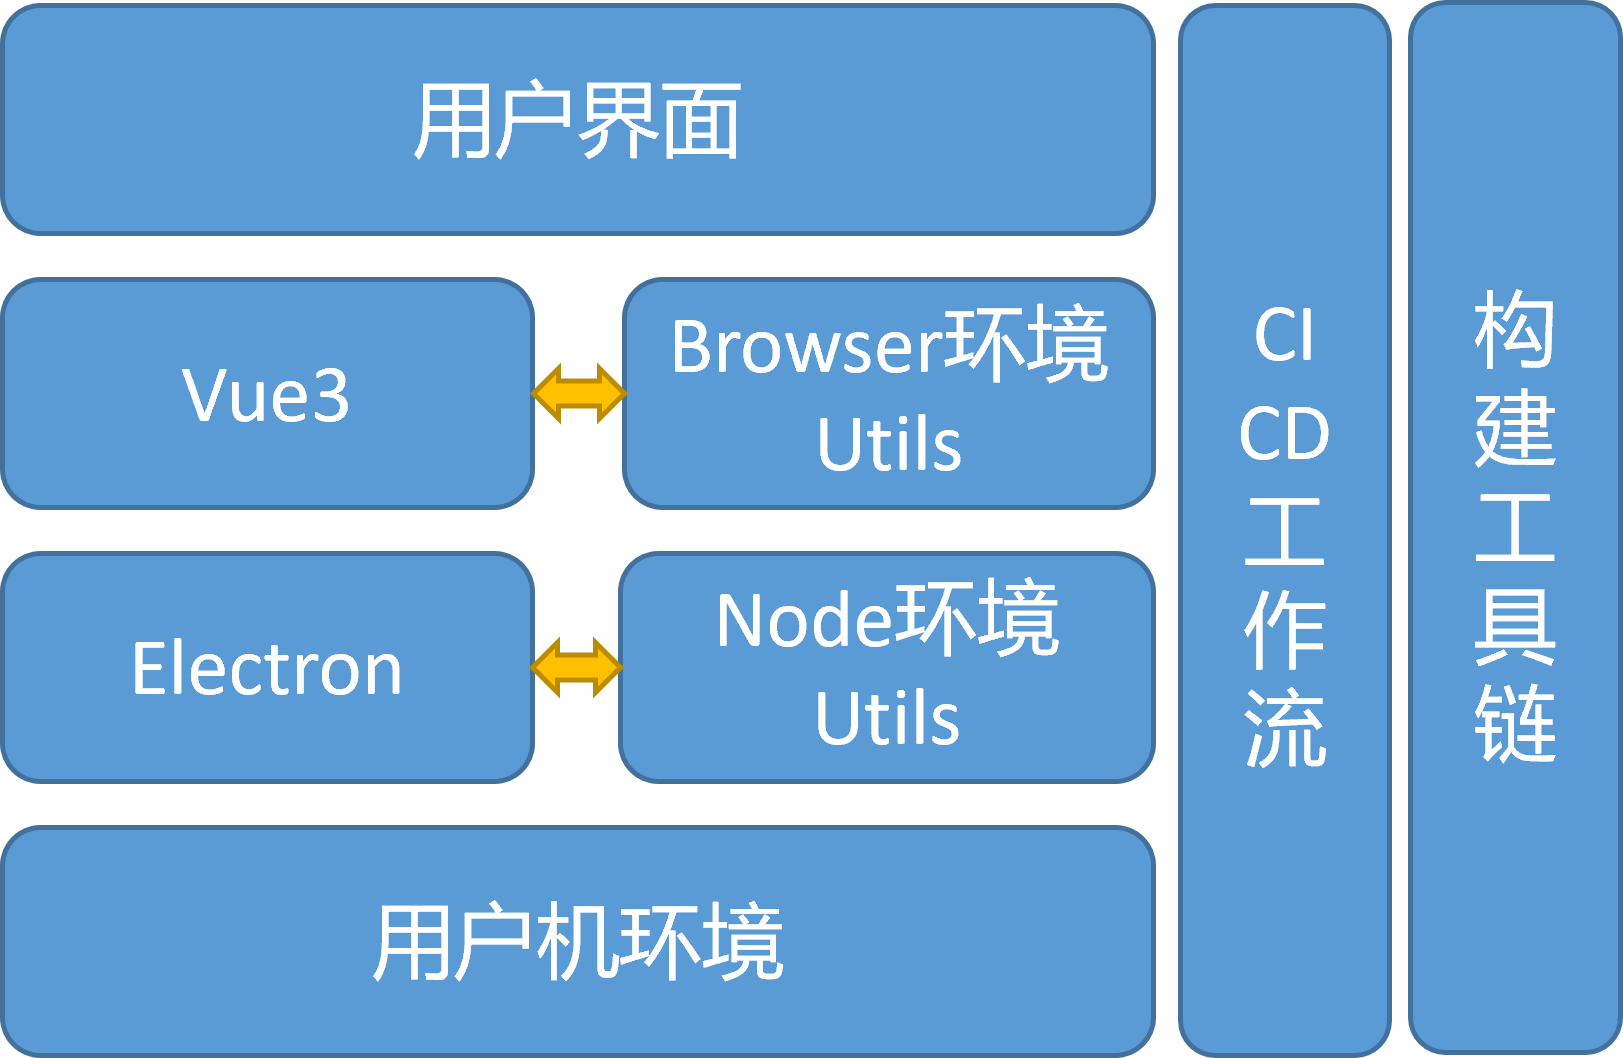
\includegraphics[scale=0.75]{figure/front_arch.png}
  \caption{\textbf{桌面端架构图}}
  \label{fig:front_arch}
\end{figure}

\figref{fig:front_arch}是PhoeniX的桌面端架构图,为了更好地解释该架构图,在此对下文中出现的一些专有名词进行解释:

\begin{enumerate}
  \item Electron:一个用于开发跨平台桌面端应用的框架,包括Visual Studio Code在内的众多软件都使用该框架进行开发,该框架的主要特色在于允许开发者使用Web开发技术开发桌面端应用。
  \item Vite:一个打包与开发Web应用的工具,在本项目中配合Electron-Builder使用,用于将Electron应用打包为应用安装包。
  \item Github Action:将软件开发过程自动化的工具,通常用于软件自动化测试、自动化部署、自动化检查等。
  \item CI/CD:全称为Continuous Integration/Continuous Deployment,即持续集成和持续部署,指软件开发中的一些自动化过程。
  \item Vue3:一个Web前端框架,通常用于网站的开发,可以配合Naive-UI等第三方组件库使用。
  \item Monaco:由微软开发的开源Web编辑器,是微软Visual Studio Code解决方案的一部分,在本项目中配合Vue3使用。
\end{enumerate}

PhoeniX桌面端将TypeScript作为主要的编程语言,相比于JavaScript,TypeScript能够提供更多的类型提示,减少代码编写中的Bug。我们采用Vite和Electron-Builder作为构建工具链,对PhoeniX进行本机调试、应用打包等操作。另外,我们使用Github Action作为核心CI/CD工作流,对PhoeniX进行自动化构建与自动化检查。PhoeniX围绕Electron框架搭建,在Electron框架之上集成了Vue3,使用Electron与用户机进行必要的交互,而使用Vue3完成主要应用逻辑的编写。PhoeniX主要使用Naive-UI构建用户界面,另外还使用了Monaco等第三方组件,提供一致而流畅的用户体验。

\section{服务端架构}

\begin{figure}[H]
  \centering
  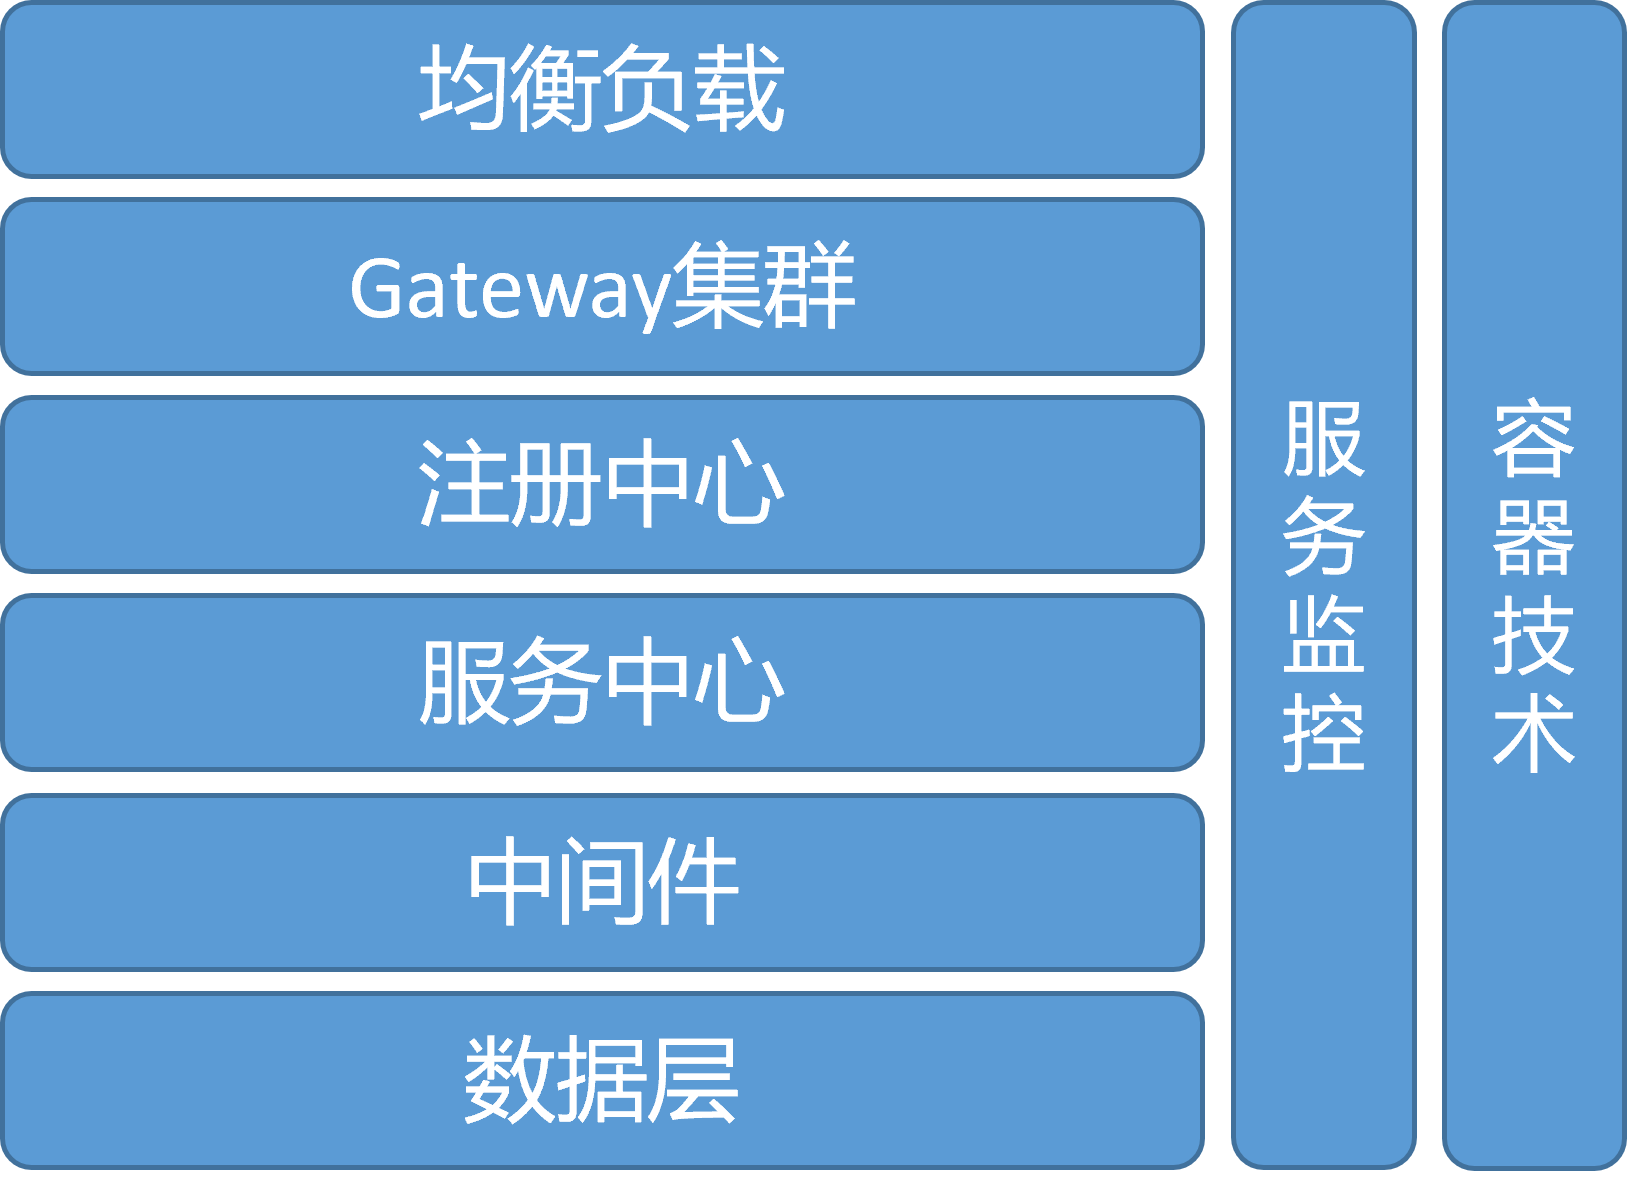
\includegraphics[scale=0.75]{figure/back_arch.png}
  \caption{\textbf{服务端架构图}}
  \label{fig:back_arch}
\end{figure}

\figref{fig:back_arch}是PhoeniX的服务端架构图,为了更好地解释该架构图,在此对下文中出现的一些专有名词进行解释:

\begin{enumerate}
  \item Kuberbetes:一个用于自动部署,扩展和管理容器化应用程序的开源系统,该系统是众多大型网站后台的首选基础设施之一。
  \item Prometheus:由SoundCloud开发的系统监控和预警工具,Prometheus也是开源软件,常用于实时监控虚拟容器的状态。
  \item LVS:Linux Virtual Server的缩写,通常用于均衡负载,将用户流量分发到不同的服务器上,重复利用服务端的资源。
  \item Etcd:提供分布式的键值对存储服务,通常用于微服务架构中的服务注册与发现,存储微服务的一些元信息。
  \item gRPC:开源高性能的RPC框架,用于各个微服务之间的相互调用,当用户的请求较为复杂时,可能需要几个微服务共同完成一个用户请求。
  \item RabbitMQ:一个消息队列,在生产者系统与消费者系统之间充当中间件,常用于对流量进行削峰,解决生产速率与消费速率不一致的问题。
\end{enumerate}

PhoeniX服务端以Golang作为主要编程语言,采用微服务架构,相比于传统的分层式架构,微服务架构能够承受更高的并发流量。我们采用Kubernetes作为服务端的运维基础,使用Prometheus对部署的各个服务进行监控。PhoeniX的服务端能够支撑高并发请求,用户流量到达服务端时,首先会到达LVS均衡负载层,均衡负载层会将请求分流到网关(Gateway)集群中的各个服务器。网关服务器提供聚合服务、路由等功能,流量经过网关服务器后到到Etcd注册中心,随后分发给对应的微服务。各个微服务采用Gin框架编写核心逻辑,使用gRPC作为RPC框架。服务中心请求数据时,将请求发送到消息中间件RabbitMQ中,不直接从MySQL等数据库中读取数据,起到流量削峰的作用。
\newpage
\chapter{项目展示}

\section{教程版块}

用户可以查看公开的以及分享给自己的教程,教程的可读权限和可写权限是在创建教程时给定的。教程支持Markdown和Latex渲染,用户可以方便地插入标题、代码块等基本元素。PhoeniX支持在教程中嵌入程序的可执行环境,用户无需打开IDE即可运行程序。教程详情页面如下:

\begin{figure}[H]
    \centering
    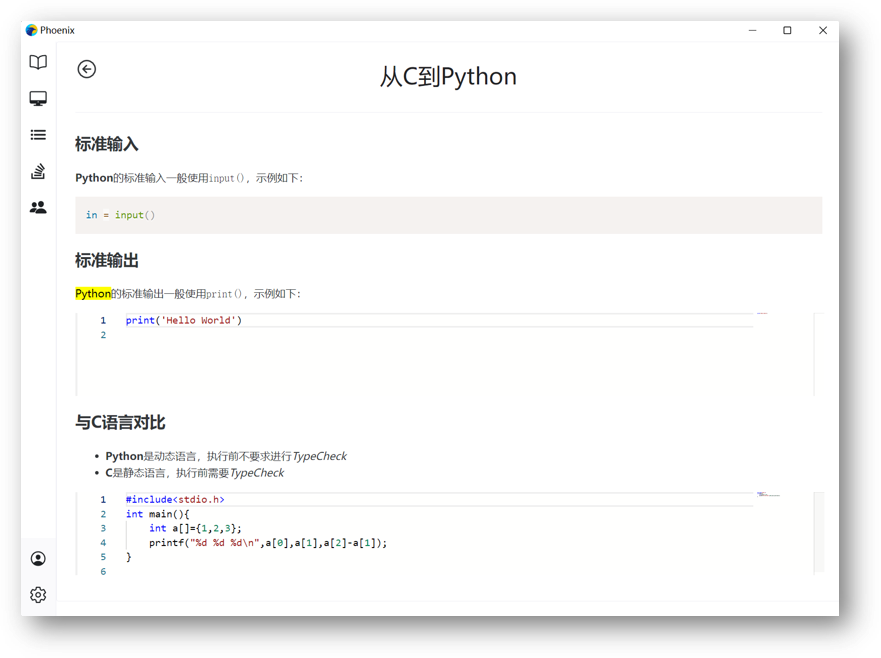
\includegraphics[width=0.7\textwidth]{figure/tutorial1.png}
    \caption{\textbf{教程详情页面}}
    \label{fig:tutorial1}
\end{figure}

\section{评测版块}

用户可以设计并上传自己的题目,并查看具有可读权限的所有题目。用户的题目列表中会标明题目的难度、名称、通过情况等信息,方便用户进行筛选,题目列表页面如下:

\begin{figure}[H]
    \centering
    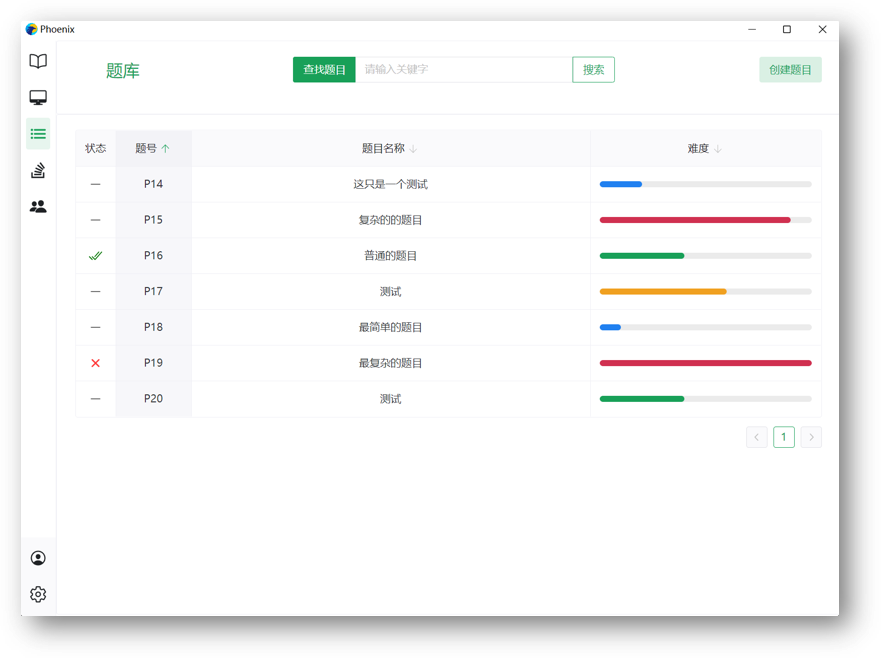
\includegraphics[width=0.7\textwidth]{figure/problem1.png}
    \caption{\textbf{题目列表页面}}
    \label{fig:problem1}
\end{figure}

对于每一个题目,用户都可以查看自己的历史评测记录。在历史评测记录中会显示用户所用的编程语言、评测结果、评测时间等信息。用户可以下载自己的历史评测文件,评测记录页面如下:

\begin{figure}[H]
    \centering
    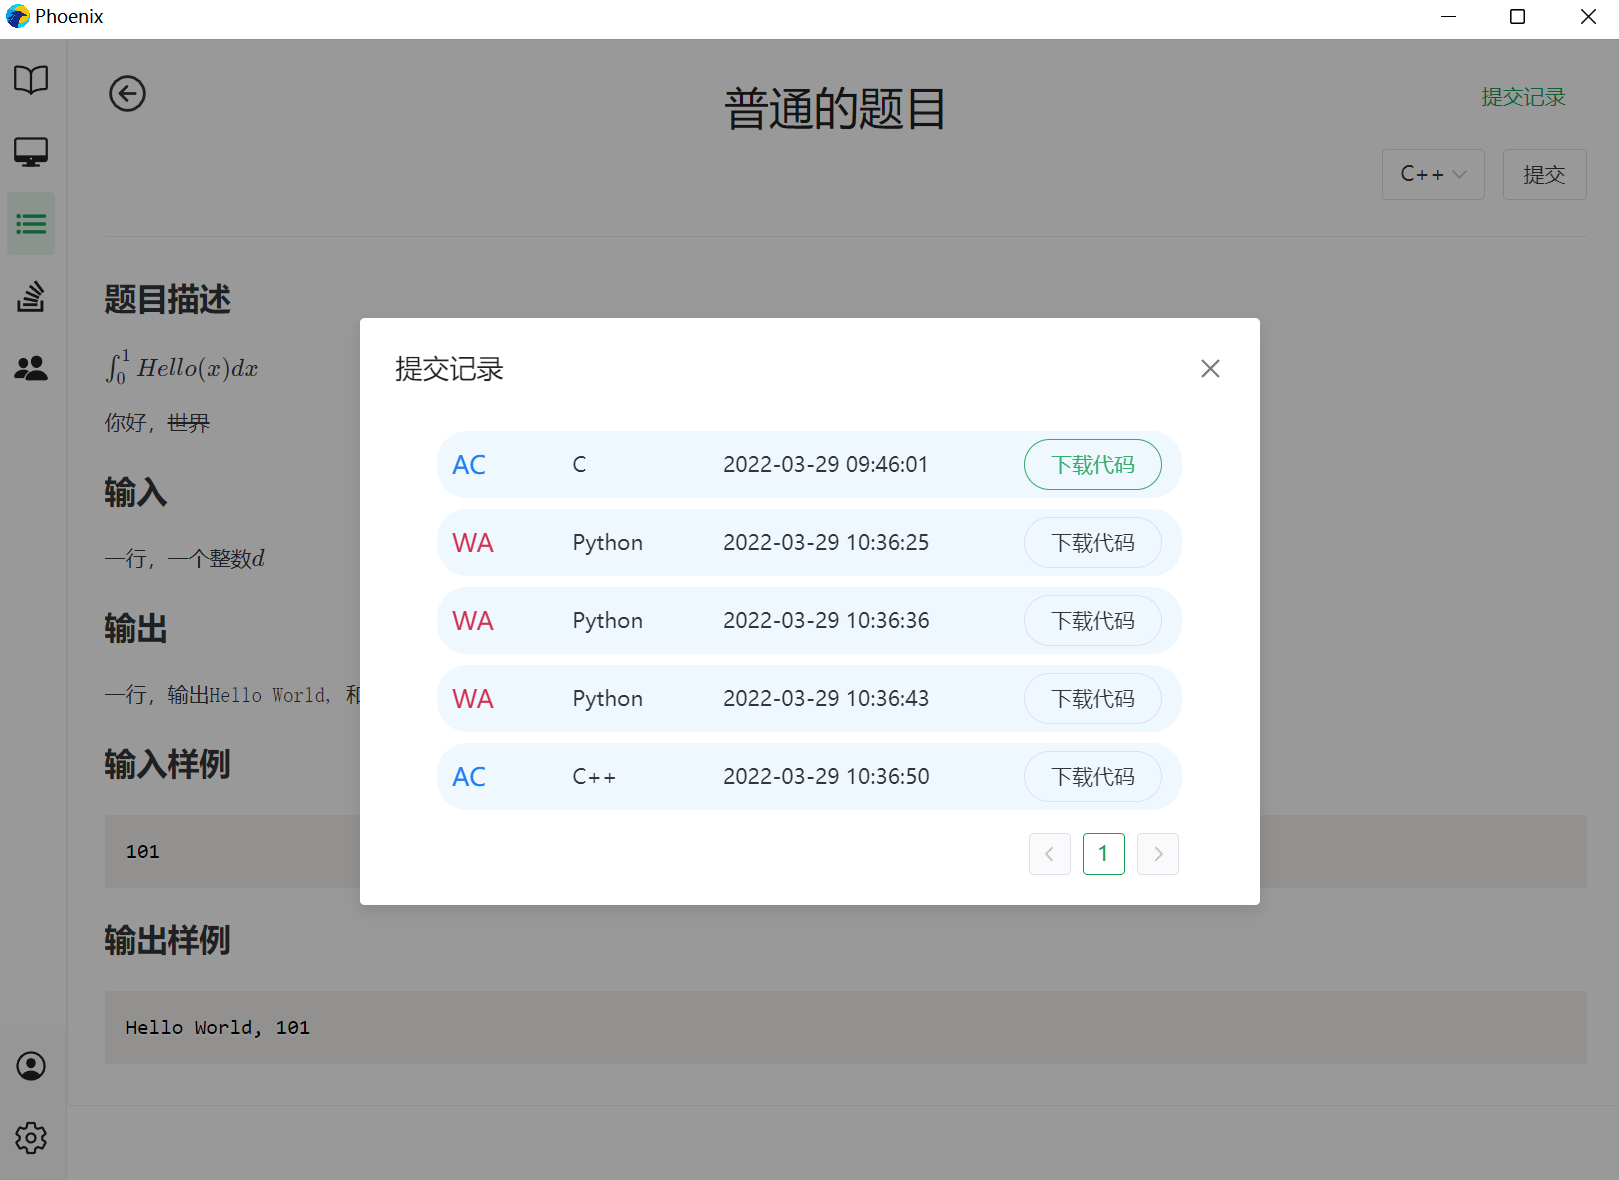
\includegraphics[width=0.7\textwidth]{figure/problem2.png}
    \caption{\textbf{评测记录页面}}
    \label{fig:problem2}
\end{figure}

\section{组织管理版块}

用户可以自发地创建组织并邀请其他用户加入,实时查看自己收到的组织邀请,并方便地查看自己所属的所有组织,组织列表页面如下:

\begin{figure}[H]
    \centering
    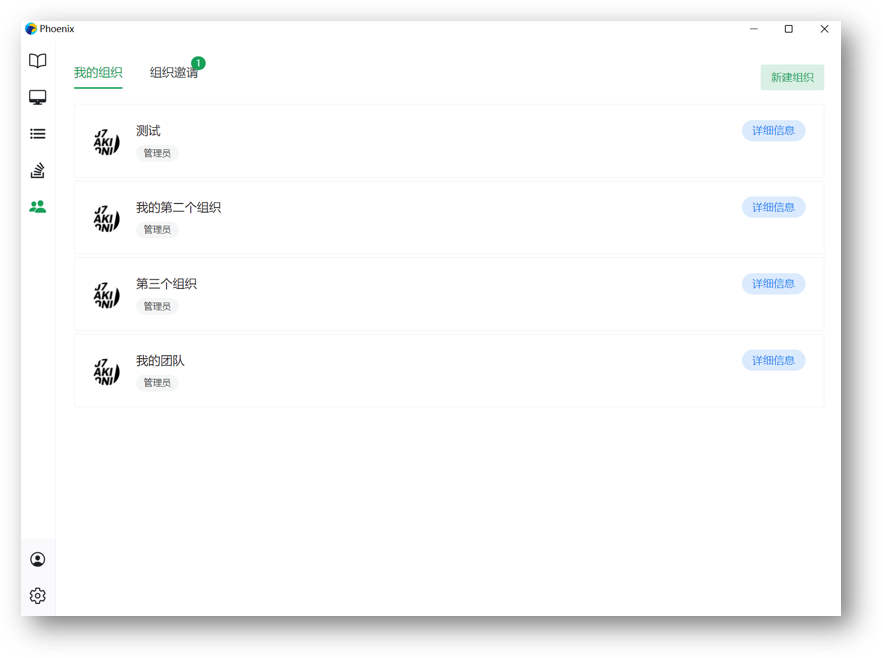
\includegraphics[width=0.7\textwidth]{figure/team1.png}
    \caption{\textbf{组织列表页面}}
    \label{fig:team1}
\end{figure}

组织创建者可以将一些组织成员设置为组织管理员。组织管理员可以设置组织的相关信息(例如组织简介等),在组织内共享题目和教程,创建组织范围内的比赛等。组织管理页面如下:

\begin{figure}[H]
    \centering
    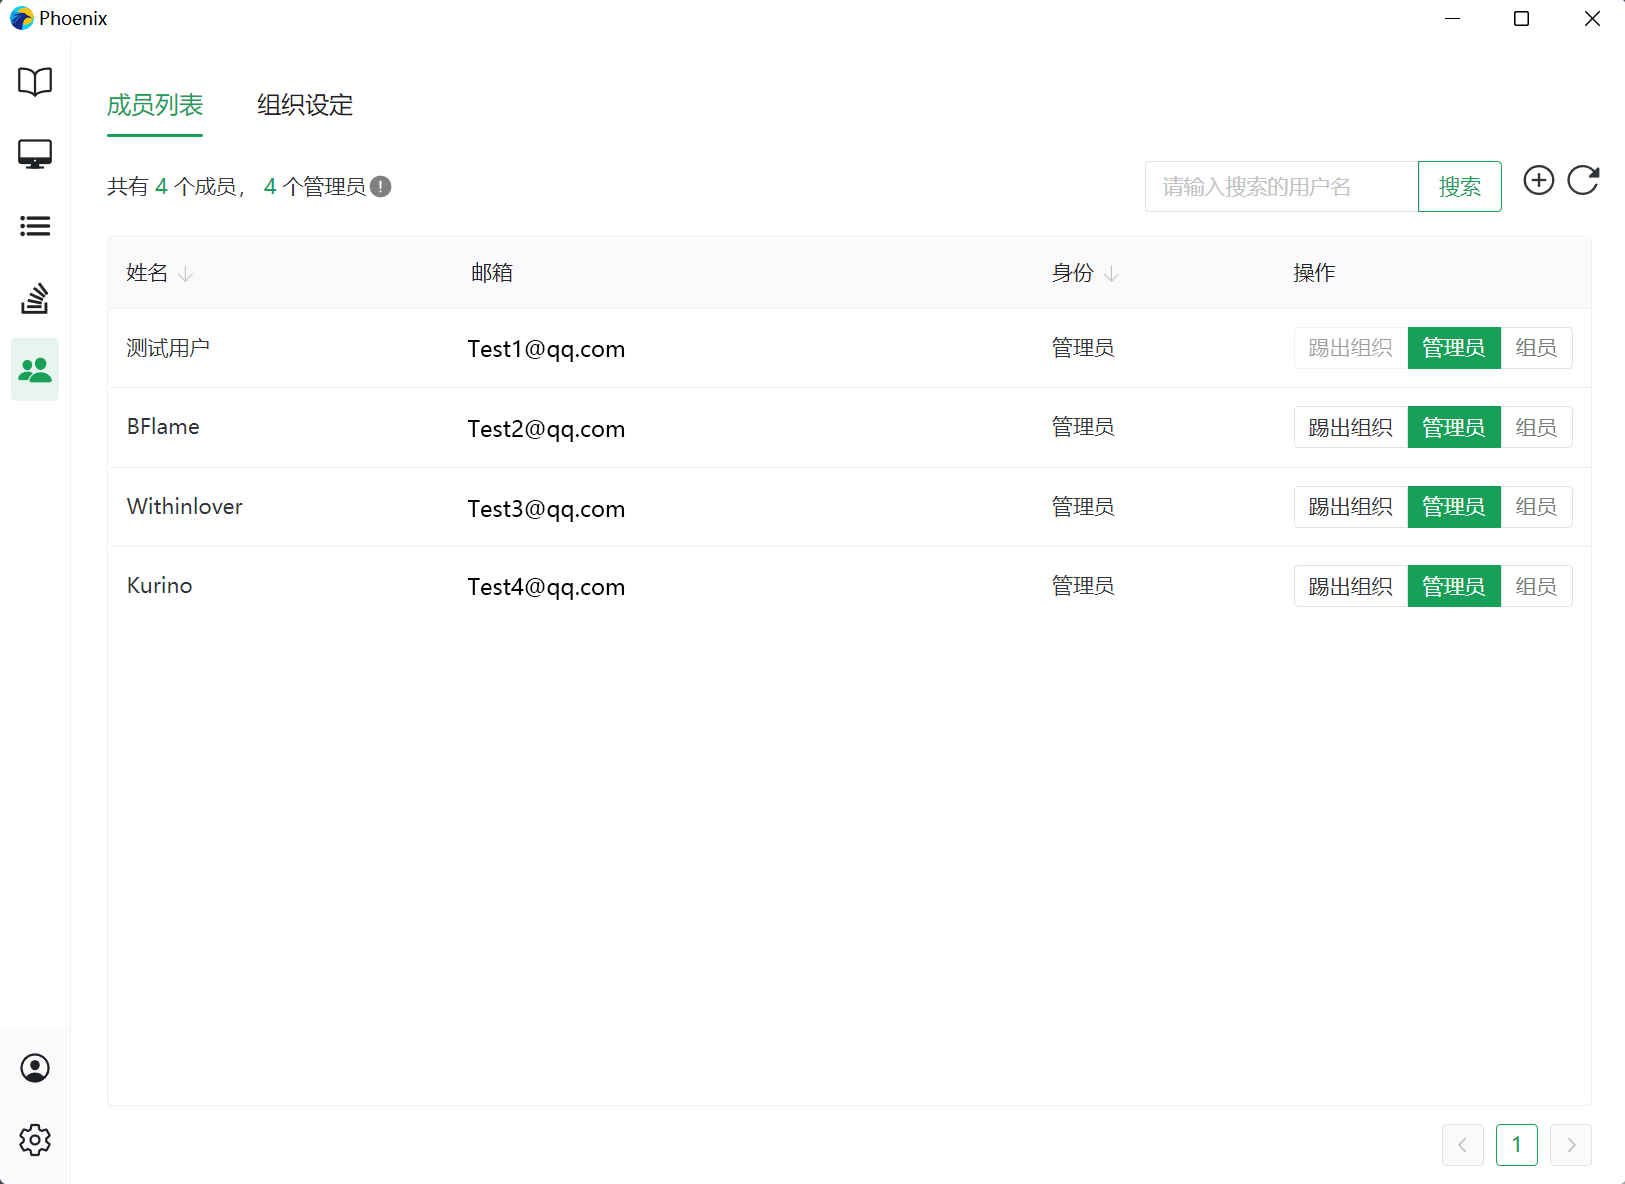
\includegraphics[width=0.7\textwidth]{figure/team2.png}
    \caption{\textbf{组织管理页面}}
    \label{fig:team2}
\end{figure}

\section{比赛版块}

组织管理员可以通过选择题目创建比赛,比赛可以指定允许参加比赛的用户范围、比赛开启的时间等内容,创建比赛页面如下:

\begin{figure}[H]
    \centering
    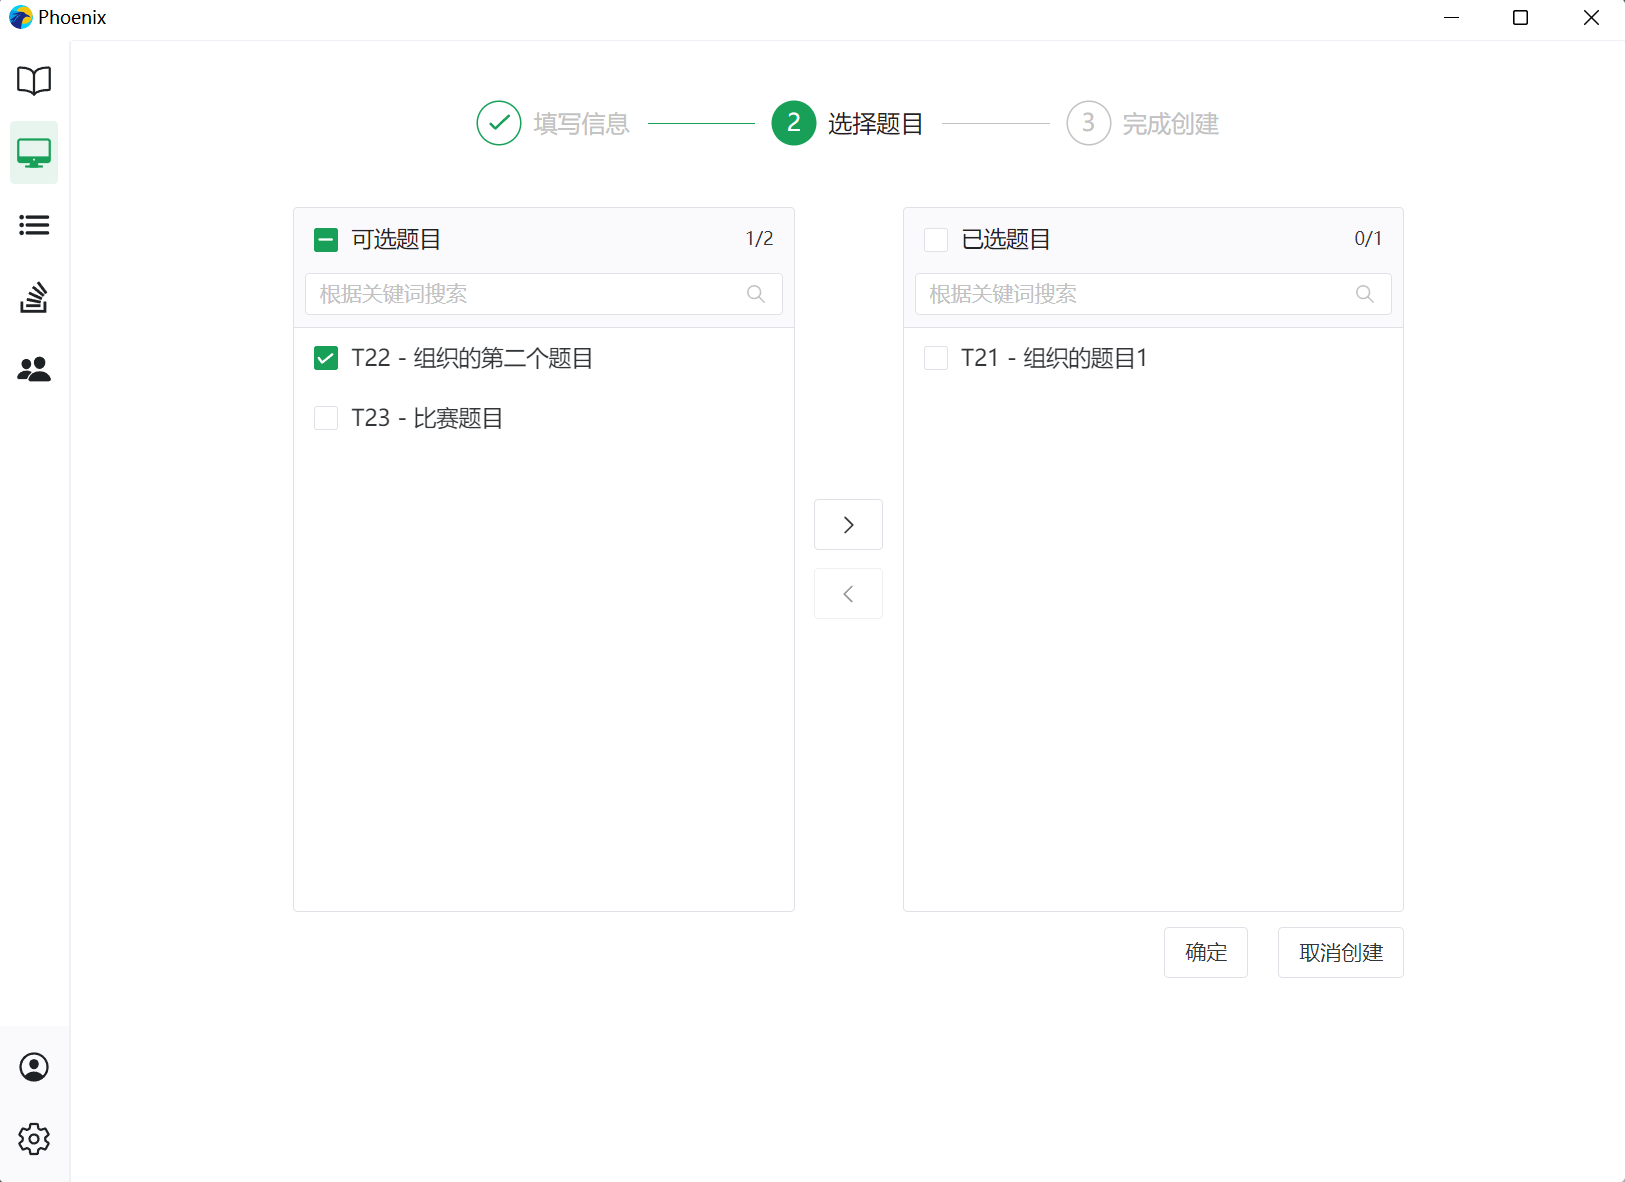
\includegraphics[width=0.7\textwidth]{figure/contest1.png}
    \caption{\textbf{创建比赛页面}}
    \label{fig:contest1}
\end{figure}

到达比赛开始的时间后,具有权限的用户可以对比赛中的题目进行提交。在比赛过程中后台将对用户的提交进行实时排名,用户可以实时看到其他用户的题目通过情况,比赛详情页面如下:

\begin{figure}[H]
    \centering
    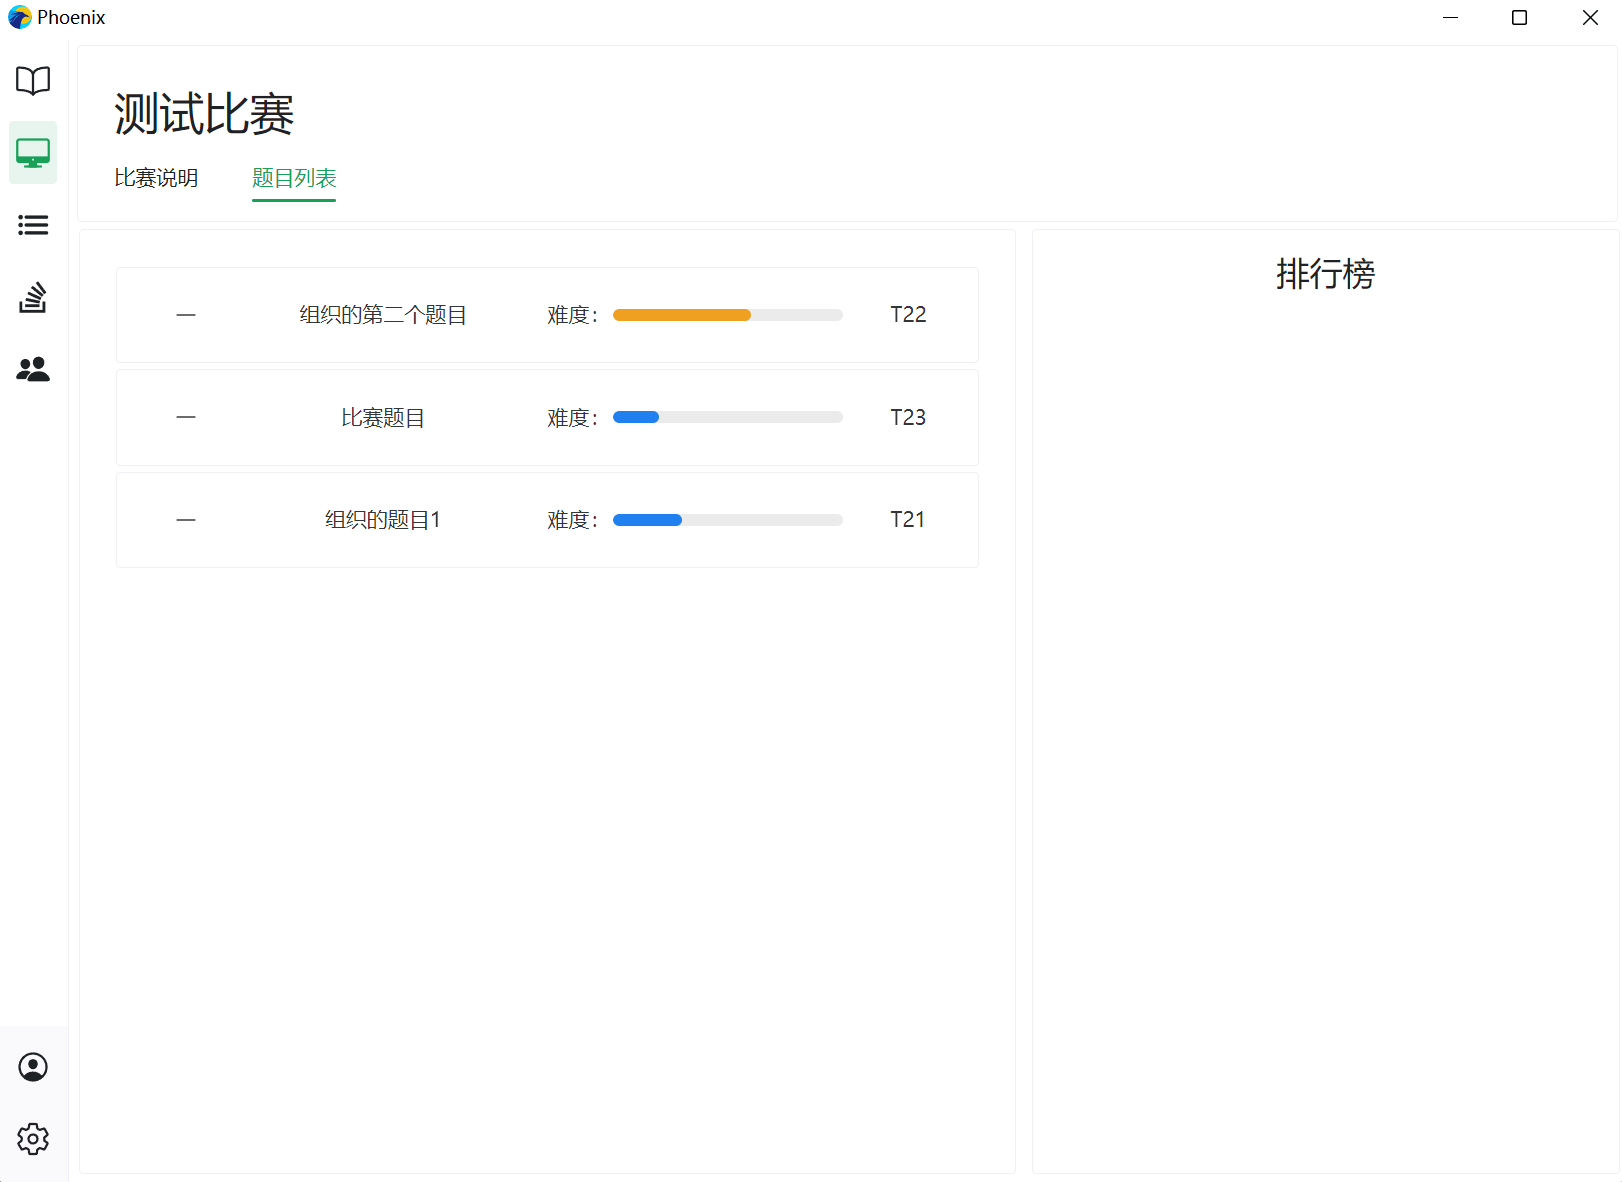
\includegraphics[width=0.7\textwidth]{figure/contest2.png}
    \caption{\textbf{比赛详情页面}}
    \label{fig:contest2}
\end{figure}

\section{论坛版块}

每个组织都有自己的论坛,组织成员可以在论坛内进行交流。论坛内置不同的版块,用于放置不同的讨论内容。论坛内的帖子和评论均可采用Markdown和Latex进行编写,并可插入图片等内容。论坛页面如下:

\begin{figure}[H]
    \centering
    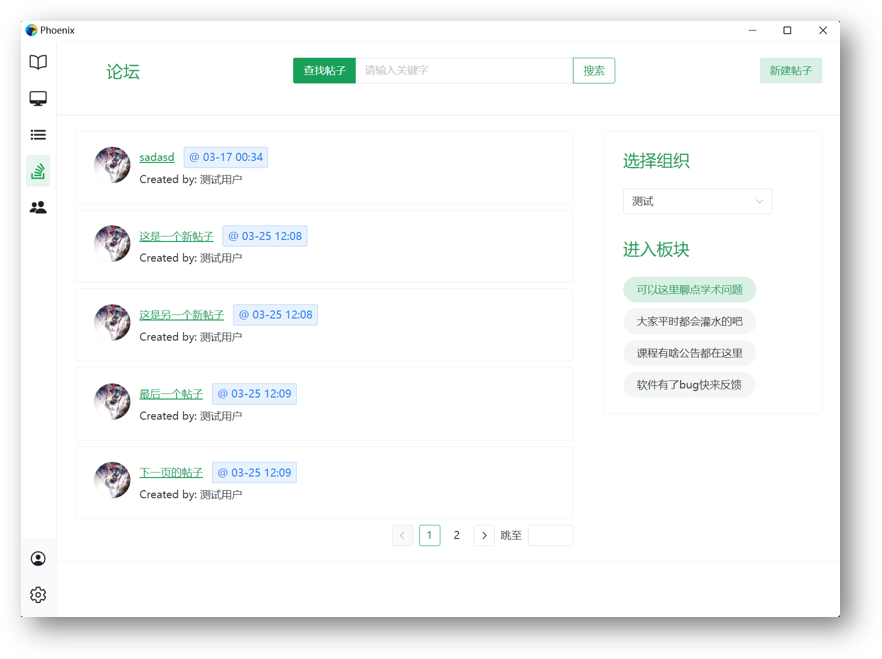
\includegraphics[width=0.7\textwidth]{figure/forum1.png}
    \caption{\textbf{论坛页面}}
    \label{fig:forum1}
\end{figure}

\newpage
\chapter{部分实现细节}

\section{评测结果的真实性}

如果用户通过某种途径(如HTTPS抓包)获取了服务端的评测接口,想通过直接调用接口的形式仿造题目评测,这是有可能的。我们在服务端对这种情况进行了处理,即用户在评测题目后会将用户的程序上传到服务端,服务端可以再次对这些代码进行评测,验证这些程序的合法性与真实性。对于组织创建的比赛,我们提供了对用户上传的程序进行查重与重测的接口,保证比赛系统的公正性。

如果人力等资源允许,事实上还可以通过训练机器学习模型,来进一步判定用户代码是否是根据题目输出编程得来的,或者是伪造的。考虑到根据题目输出编程得来的程序的特征(源代码中包含大量标准输出),使用正则表达式匹配就能筛选出大部分这类程序。这一部分的工作我们仍处于筹划阶段,具体实现方法仍待考虑。

\section{教程的渲染}

PhoeniX给用户呈现的教程需要能够嵌入代码执行环境,渲染Latex公式以及Markdown语法,保证渲染后的教程对用户而言没有安全风险。经过考量之后,我们选用了以markdown-it渲染器为核心的渲染方案,原因有如下几点:

\begin{enumerate}
    \item 教程的渲染需要较高的效率,而且之后可能需要支持更多的语法与渲染内容,引入第三方封装的markdown编辑器做渲染是明显不合适的,这些编辑器的渲染效率不高,且难以自定义渲染效果。
    \item markdown-it渲染器本身足够轻量,使用者和维护者都较多,能够识别并正确渲染HTML保证用户安全,且支持自定义插件,容易自定义渲染效果。
    \item markdown-it有一些现成的足够轻量的插件,分别能够支持Latex渲染、Markdown扩展语法渲染等任务,不需要重新手写太多插件。
\end{enumerate}

然而,markdown-it渲染器只能完成最基本的渲染任务,对于内嵌的代码执行环境,我们是使用Monaco编辑器和Xterm虚拟终端实现的。Monaco编辑器和Xterm终端是微软的开源项目Visual Studio Code(以下简称VSCode)解决方案的一部分,考虑到VSCode给用户提供的绝佳体验,我们认为VSCode的编辑器解决方案是成功的。在PhoeniX的具体实现上,我们对Monaco和Xterm都进行了一定程度的自定义,使其能够较为美观的呈现,并保有执行我们提供的命令的基本功能。

\section{推荐算法的设计}

我们设计了一套基于情景感知的题目推荐模型。我们的设计理念是要尽可能地推荐用户最有可能查看并完成的题目。即,规定事件 $X$ 为用户对于某个题目的提交。$Y$ 表示用户当前的“情景”。其构成包括:用户近期所做过的题目、题目标签、题目难度、用户所属的组织、组织成员的做题偏好等。我们的目标则是最大化 $P(X|Y)$。

具体而言,我们针对特定情境寻找题目时,会计算下列信息:

\begin{enumerate}
    \item 提取出用户近期提交过的题目标签。提升拥有相同标签的题目的权重。
    \item 根据用户最近过题的难易程度,降低难度较高或较低的题目权重。
    \item 查看用户所属组织成员的做题情况,提升组织内其他成员做过的题目的权重。
    \item 系统内预设一套学习路线,根据学习路线预测用户接下来可能学习的知识点。提升其模板题的权重。
\end{enumerate}

我们将题目按照权重排序,选择权重最高的题目返回给用户,实现个性化的推荐功能。此外,我们还会全局统计每个题的近期过题量,找出近期的热门题目,以排行榜的形式展示。这也可以作为用户选择题目的参考。

在具体的实现中,由于不同影响因素的重要程度难以衡量,我们会尽可能的给用户更多样化的选择,具体而言。当有很多权重很高的题目时,我们会随机删除掉部分权重很高但是题目标签重复出现的题目。来保证我们推荐的题目的多样性。
\newpage
\chapter{前景展望}

\section{项目已取得的成果}
\begin{enumerate}
    

\item{教学测一体化的平台}
\par
本项目PhoeniX是使用Electron框架搭建的桌面端应用,针对学生在学习校内课程各类资源或是评测网站过于分散的问题进行开发,集教程、评测、社交于一体,为学生搭建了一个方便使用、评测快捷、促进交流的学习环境。
\item{多语言分布式评测}
\par
PhoeniX因为其桌面端软件的优越性,相比传统的评测网站可以为用户提供分布式评测的功能,并有效降低中心服务器的评测压力。只要在远程配置不同题目的评测脚本,就让用户的评测程序在PhoeniX提供的本地环境下编译并运行,并在本地给出评测的结果。因为程序在本地编译运行的方法,PhoeniX还支持更复杂的多文件、多语言评测的功能,让评测的程序种类有了更多可能。

\item{可交互式的教程}
\par
PhoeniX的教程设计哲学与JupyterBook一致,其所有交互计算、编写说明文档、数学公式、图片以及其他富媒体形式的输入和输出,都是以文档的形式体现的。教程编写者只需要撰写一份带有标记格式的文档,在PhoeniX中就可以被解析为一篇支持代码缩进高亮、编译执行的教程页面,供教程学习者自由学习和实验。
\item{组织管理与个人表达}
\par
在课程教学和各类算法竞赛的实践中,学生往往有在编程时组队、实时排名的需求。因此PhoeniX让用户可以自由创建组织,并在组织内分享比赛和教程。在教学实践中,对于一些教程和竞赛的开放权限也可以通过组织成员的权限管理轻松在班级中投送内容。除此之外,学生在学习中遇到的困难或是想要分享的技术都可以在公开的论坛或是组内进行讨论。
\end{enumerate}
\newpage

\section{项目仍存在的问题}
\begin{enumerate}
    \item 项目仍在更新开发状态,每次迭代更新后的新版本发布后需要用户重新下载。
    \item UI的排版和易用性上还有优化的空间。
    \item 使用Electron框架导致安装包体较大,会考虑缩减一些不必要的依赖。
\end{enumerate}
\section{未来的目标}
对于未来版本的PhoeniX的升级计划,我们的目标如下:
\begin{enumerate}
    \item 引入智能推荐的系统。根据用户近期的做题情况,查看教程情况,量身定制推荐题库及教程。
    \item 搜索结果的智能排序。用户在搜索教程/问题时,按照教程/问题的权重进行排序,并返回给用户。
    \item 自动化的上传内容审查。用户上传教程/问题时,自动对内容进行审核,提高平台智能化程度。
\end{enumerate}
我们希望PhoeniX提供的教学测平台的一体化解决方案能够真正地优化同学们在学习编程和算法时的体验。

\newpage
\markboth{结论}{结论}
\addcontentsline{toc}{chapter}{结论} % 添加到目录中

\chapter*{结论}
本项目PhoeniX设计并实现了一个集编程教学、在线评测、轻社交等为一体的编程学习平台。PhoeniX解决了在编程学习中各类资源与评测网站过于分散、用户等待题目评测的时间过长等痛点问题,使用了最新的前后端技术栈进行开发,为编程学习者创造了一个知识充分共享、评测体系完备、团队交流友好的学习环境。

与当前北航学生使用的评测软件与网站相比,PhoeniX兼具美观易用的GUI界面与分布式评测的能力,可以在提升学生用户编程学习与评测体验的同时,有效减轻中心服务器的负载压力。

用户社区和教程模块也是PhoeniX最大的特色之一。通过团队、论坛的自由组建,用户可以在团队内或论坛分享自己学习的心得与经验。并且借助实时可编辑、可执行的代码的教程展示,可以让编程学习者能够更直观地体会到编码的要领。

在未来,为了优化用户的体验,PhoeniX将在题目与教程系统中引入智能推荐,个性化用户的学习需求。另外,还将在上传内容方面进行自动化审查,提高平台的安全与智能化程度。

\par


\clearpage

%%%%%%%%%%  参考文献  %%%%%%%%%%
\bibliographystyle{references/FengruCupStyle}
\markboth{参考文献}{参考文献}
\addcontentsline{toc}{chapter}{参考文献}
\nocite{*}
\bibliography{references/ref}


%%%%%%%%%%   附录   %%%%%%%%%%

% \include{appendix/material}
% \include{appendix/code}

% % 重新设置想要的chapter格式
% \titleformat{\chapter}{\raggedright\sihao\hei}{\chaptername}{2em}{}

\clearpage
\end{CJK*}
\end{document}